% Fig 1 — LoD verification planning pipeline with folklore failure ports (v2)
\documentclass[tikz,border=3pt]{standalone}
\usepackage[T1]{fontenc}
\usepackage{helvet}
\renewcommand{\familydefault}{\sfdefault}
\usetikzlibrary{arrows.meta,positioning,fit,backgrounds,calc}

\definecolor{lodblue}{HTML}{2166AC}
\definecolor{lodorange}{HTML}{D95F02}
\definecolor{lodpurple}{HTML}{762A83}
\definecolor{lodgray}{HTML}{636363}
\definecolor{loddash}{HTML}{B0BEC5}
\definecolor{lodred}{HTML}{B2182B}
\definecolor{lodgreen}{HTML}{1B7837}

\tikzset{
  stage/.style={
    draw=#1, thick, rounded corners=2pt, fill=white,
    minimum height=7.5mm, minimum width=14mm, align=center,
    font=\footnotesize, inner sep=2pt
  },
  goal/.style={stage=#1, minimum width=17mm},
  arr/.style={-{Stealth[length=2mm]}, draw=lodgray, thick},
  arrD/.style={-{Stealth[length=2mm]}, draw=loddash, thick, dashed},
  arrW/.style={-{Stealth[length=2mm]}, draw=lodorange, thick, dashed},
  port/.style={
    draw=lodred, thick, rounded corners=1.5pt, fill=lodred!6,
    font=\scriptsize, text=lodred, align=center, inner sep=2pt
  },
}

\begin{document}
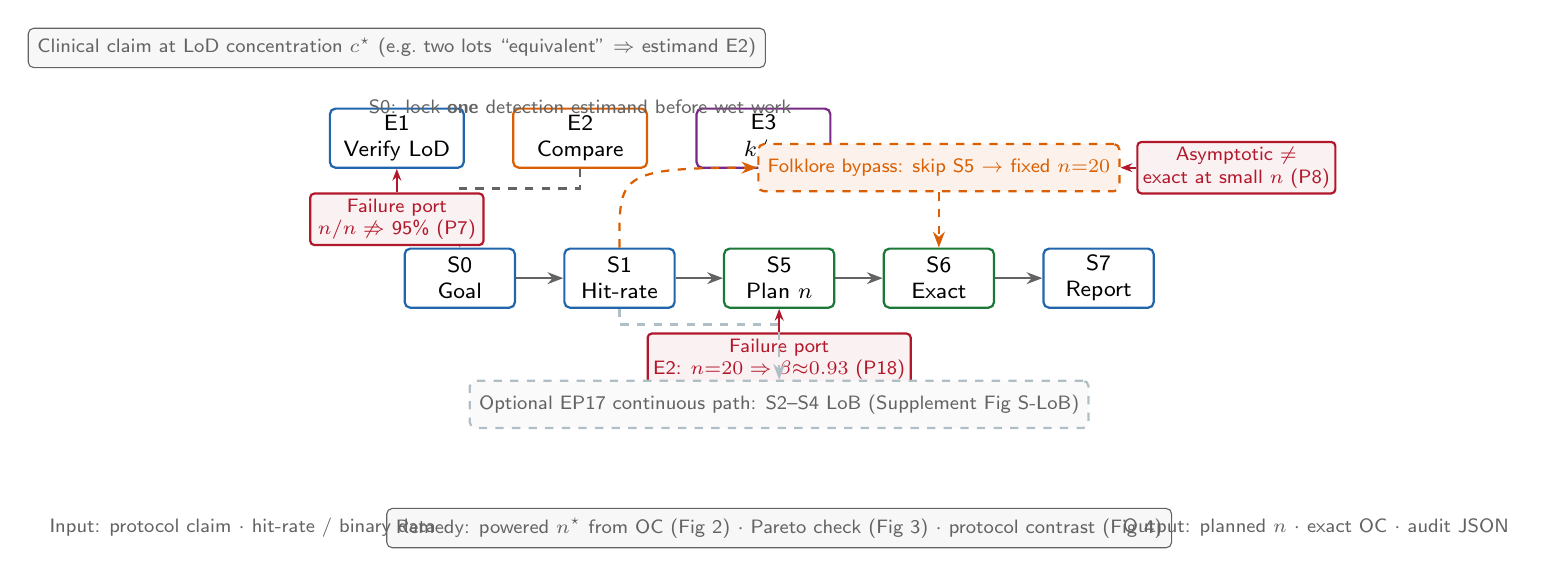
\begin{tikzpicture}[node distance=4mm and 6mm]

  % Clinical anchor
  \node[draw=lodgray, fill=black!3, rounded corners=2pt,
        minimum width=88mm, minimum height=5mm,
        font=\scriptsize, text=lodgray] (claim)
        {Clinical claim at LoD concentration $c^\star$ (e.g.\ two lots ``equivalent'' $\Rightarrow$ estimand E2)};

  % E1 / E2 / E3 (LoD scope)
  \node[goal=lodblue, below=5mm of claim] (g1) {E1\\Verify LoD};
  \node[goal=lodorange, right=of g1] (g2) {E2\\Compare};
  \node[goal=lodpurple, right=of g2] (g4) {E3\\$k/n$};
  \node[above=0mm of g2, font=\scriptsize, text=lodgray, yshift=-2mm]
        {S0: lock \textbf{one} detection estimand before wet work};

  % Main LoD pipeline
  \node[stage=lodblue, below=10mm of g1, xshift=8mm] (s0) {S0\\Goal};
  \node[stage=lodblue, right=of s0] (s1) {S1\\Hit-rate};
  \node[stage=lodgreen, right=of s1] (s5) {S5\\Plan $n$};
  \node[stage=lodgreen, right=of s5] (s6) {S6\\Exact};
  \node[stage=lodblue, right=of s6] (s7) {S7\\Report};
  \foreach \a/\b in {s0/s1,s1/s5,s5/s6,s6/s7}
    \draw[arr] (\a) -- (\b);

  \draw[arr, dashed] (g2.south) -- ++(0,-2.5mm) -| (s0.north);

  % --- Mechanism: folklore bypass (failure path) ---
  \node[draw=lodorange, dashed, thick, rounded corners=2pt, fill=lodorange!8,
        minimum width=36mm, minimum height=6mm, above=7mm of s6,
        font=\scriptsize, text=lodorange, align=center] (bypass)
        {Folklore bypass: skip S5 $\rightarrow$ fixed $n{=}20$};

  \draw[arrW] (s1.north) .. controls +(0,9mm) and +(-18mm,0) .. (bypass.west);
  \draw[arrW] (bypass.south) -- (s6.north);

  % --- Failure ports (where fixed SOPs break) ---
  \node[port, below=3mm of g1, minimum width=22mm] (p7)
        {Failure port\\$n/n \not\Rightarrow$ 95\% (P7)};
  \draw[-{Stealth[length=1.5mm]}, draw=lodred, thick] (p7.north) -- (g1.south);

  \node[port, below=3mm of s5, minimum width=26mm] (p18)
        {Failure port\\E2: $n{=}20 \Rightarrow \beta{\approx}0.93$ (P18)};
  \draw[-{Stealth[length=1.5mm]}, draw=lodred, thick] (p18.north) -- (s5.south);

  \node[port, right=2mm of bypass, minimum width=24mm] (p8)
        {Asymptotic $\neq$\\exact at small $n$ (P8)};
  \draw[-{Stealth[length=1.5mm]}, draw=lodred, thick] (p8.west) -- (bypass.east);

  % Optional continuous / LoB branch (supplement)
  \node[draw=loddash, dashed, thick, rounded corners=2pt, fill=black!2,
        minimum width=42mm, minimum height=6mm, below=9mm of s5,
        font=\scriptsize, text=lodgray, align=center] (sup)
        {Optional EP17 continuous path: S2--S4 LoB (Supplement Fig S-LoB)};

  \draw[arrD] (s1.south) -- ++(0,-2mm) -| (sup.north);

  % Audit strip
  \node[draw=lodgray, fill=black!3, rounded corners=2pt,
        minimum width=92mm, minimum height=5mm,
        below=10mm of sup, font=\scriptsize, text=lodgray] (audit)
        {Remedy: powered $n^\star$ from OC (Fig~2) $\cdot$ Pareto check (Fig~3) $\cdot$ protocol contrast (Fig~4)};

  \node[font=\scriptsize, text=lodgray, anchor=west] at ([xshift=-44mm]audit.west)
        {Input: protocol claim $\cdot$ hit-rate / binary data};
  \node[font=\scriptsize, text=lodgray, anchor=east] at ([xshift=44mm]audit.east)
        {Output: planned $n$ $\cdot$ exact OC $\cdot$ audit JSON};

\end{tikzpicture}
\end{document}
